\chapter{OpenSITEM: Sistema Federado de Aplicaciones para la Caracterización de Nodos Potenciales de Redes de e-salud}

\textbf{OpenSITEM }es un sistema federado de aplicaciones de software libre o de código abierto que provee herramientas para analizar datos e información de los siguientes elementos que son de interés para la descripción - y definición de capacidad de, nodos potenciales de redes de e-salud: entidades de salud, servicios médicos, tecnologías de interconexión, operadores de telecomunicaciones, equipos médicos, organizaciones, profesionales, estándares, pacientes, enfermedades, medicamentos y proyectos. Provee un ambiente para apoyar las tareas de las comunidades de práctica involucradas en la investigación, el diseño, mantenimiento, desarrollo e implementación de redes de eSalud. Tuvo su génesis conceptual en la primera fase del Proyecto Telemedicina Bogotá como solución a la necesidad de administrar los resultados del estudio de campo realizado a las entidades e instituciones de salud y los operadores de Telecomunicaciones en la ciudad de Bogotá.

Su principal objetivo es: Implementar un sistema que permita la definición, categorización y caracterización de nodos potenciales de redes de eSalud, para apoyar las actividades básicas de los \textit{trabajadores del conocimiento} en el área de la telemedicina del grupo GITEM\footnote{Conformado por profesionales y estudiantes de la Universidad Distrital así como por profesionales de las diferentes instituciones que han participado en los diferentes estudios de campo.}  ofreciéndoles, además de un repositorio de datos, herramientas que facilitan las tareas de capturar, extraer, organizar, analizar, encontrar, sintetizar, distribuir y compartir información y conocimiento de nodos potenciales de las redes de eSalud. OpenSITEM cuenta con herramientas para poder  actualizar el estado de los nodos definods en el modelo base así como para la definición de nodos y categorías inéditas del Sistema de Salud de Bogotá Distrito Capital. El modelo base de nodos y categorías se construye a partir del estudio de campo realizado por el grupo de investigación, haciendo especial énfasis en los requerimientos de eSalud que se definieron en esa época. 
\begin{figure}
 \centering
 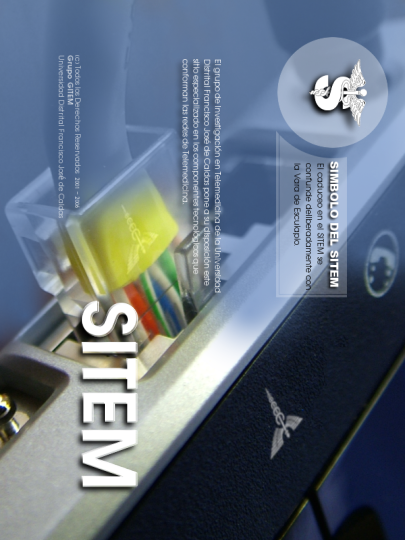
\includegraphics[width=142mm, height=190mm]{sitem_principal.png}
 \caption{Imagen en el año 2017 del Sistema de Información para Proyectos de Telemedicina}
 \label{pantalla_sitem}
\end{figure}


% ---- Fin revisión 2018/01/12








Con el SITEM se disminuye el tiempo de adquisición, análisis y despliegue de la información. Es construido guiado por adaptaciones de procesos de desarrollo ampliamente conocidos \cite{koch}\cite{jacobson2000}\cite{larman2004} y siguiendo el paradigma de la orientación a objetos con lo que se garantiza su facilidad de mantenimiento, escalabilidad e indirectamente su permanencia en el medio.

Contiene módulos para la generación de estadísticas e informes pormenorizados de cada uno de los componentes y logra obtener en unos pocos segundos los datos necesarios para apoyar la labor de análisis, diseño e implementación de proyectos telemédicos o de telesalud. Usa un esquema modular de crecimiento a la medida en donde el esfuerzo para la creación de instrumentos nuevos de consulta se minimiza por el uso de plantillas prediseñadas. En lugar de ser un Sistema estático, SITEM contiene características de adaptación dinámica para cubrir las necesidades que tengan los próximos proyectos emanados del GITEM y otras entidades que hagan uso del sistema\footnote{El modelo y patrones de desarrollo del SITEM son actualmente usados en la construcción de portales de información institucional y en el Sistema Informático de Apoyo a la Evaluación que se encuentra desplegado en varias universidades.}.

El sistema gestiona la estructuración de encuestas, formularios y talleres para crear un mecanismo ágil y costo - efectivo de recolección de información para las etapas de descripción y explicación\cite{hurtado2000} en proyectos de Telemedicina. Debido a que los resultados de los análisis pueden ser compartidos, sirven de guía a las instituciones o personas que deseen realizar estudios similares acerca del tema, facilitando el estudio de casos.

\section{Características innovadoras del SITEM}

El SITEM es el primer Sistema de Información de \textit{acceso público} en el entorno colombiano que gestiona información de la mayoría de los componentes fundamentales de las redes de Telemedicina, dotando a la comunidad de una herramienta única en su género, la cual puede ser utilizada en todas las etapas de desarrollo de proyectos en Telemedicina. Dentro de las múltiples ventajas que ofrece el sistema es que facilita la obtención de información ubicua y en tiempo real, lo que es indispensable para el apoyo óptimo en la toma de decisiones. 

El desarrollo mismo del SITEM se convierte en un modelo a seguir para proyectos básicos de Telemedicina o Telesalud orientados a la Web proponiendo una arquitectura de desarrollo interoperable, escalable y fundamentada en software libre. La integración de tecnologías Web en el SITEM brinda una plataforma robusta para la implementación de servicios en entidades de salud que carezcan de altos recursos financieros. Esto a mediano plazo podrá generar un crecimiento de la oferta de servicios de medicina a distancia\cite{itu}\cite{craig2005}, ya que ayuda a mejorar la relación costo/beneficio en proyectos que por estar fundamentados en software comercial hasta el momento han sido inviables. 

Con la puesta en marcha del proyecto SITEM se capta la atención del usuario en salud para que conozca y entienda las posibilidades de la tecnología de Telemedicina y empiece a tomar un papel activo en el desarrollo y despliegue de esta opción de servicio.

\section{Arquitectura del Sistema}

SITEM es implementado sobre una arquitectura multicapa que distribuye los diferentes componentes en tres capas principales: Presentación, aplicación y datos, estando presente una capa transversal tácita de seguridad. A nivel de usuario el SITEM está compuesto por siete subsistemas autónomos, figura \ref{componentes_sitem}, que prestan servicios a sus pares. Estos agrupan seis componentes claves en todo proyecto de telemedicina: entidades de salud, operadores de telecomunicaciones, tecnologías de interconexión, equipos y tecnologías de captura de datos, proyectos e instituciones relacionadas con la telemedicina y servicios médicos - incluyendo módulos de vademécum, consulta de procedimientos, enfermedades y especialidades médicas.

\begin{figure}
 \centering
 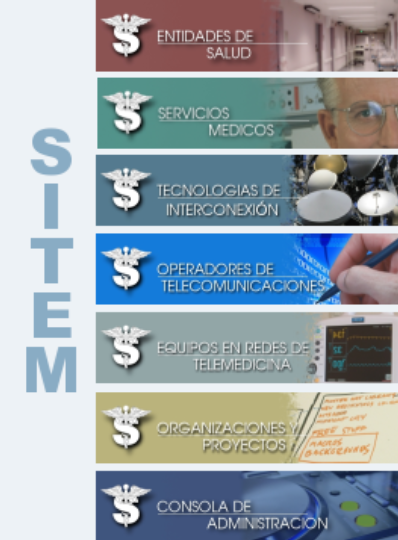
\includegraphics[width=140mm, height=190mm]{componentes_sitem.png}
 \caption{Subsistemas Principales del SITEM}
 \label{componentes_sitem}
\end{figure}


\subsection{Subsistema Entidades de Salud} 
Este subsistema, figura \ref{entidades}, se creó para gestionar los datos recopilados en el estudio de campo realizado por el grupo GITEM en el marco del proyecto del Sistema de Gestión de Salud para el Distrito Capital fases I y II. Es por ende el subsistema base para el SITEM y su objetivo principal es la gestión de información referente a las entidades de salud en el entorno colombiano enfocándose en tres redes principales: la red de especialidades médicas, la red de comunicaciones y la red de atención.

\begin{figure}
 \centering
 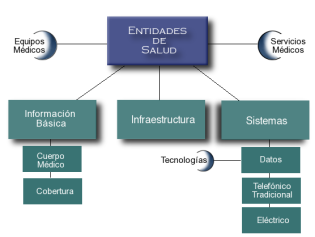
\includegraphics[width=80mm, height=52mm]{entidades.png}
 \caption{Arquitectura Básica del Subsistema Entidades}
\label{entidades}
\end{figure}

La información disponible en el subsistema puede ser administrada por cada una de las entidades prestadoras de servicios de salud, de tal forma que se cree gradualmente un catálogo flexible para conocer el estado actual de las entidades y su potencialidad para ser parte en redes que presten servicios de salud a distancia usando TIC. Por defecto, las entidades se asocian a la arquitectura de red de la secretaría de Salud de Bogotá pero por medio del módulo denominado \textit{redes de atención} se puede crear fácilmente cualquier prototipo de red jerárquica de atención \cite{yellowlees}.

\subsection{Subsistema Tecnologías de Interconexión} 
Administra información relacionada con las tecnologías y protocolos de interconexión disponibles en las redes de acceso y transporte. Estas tecnologías se ordenan principalmente sobre el modelo de referencia OSI pudiéndose crear  - desde el módulo de arquitecturas, cualquier otro tipo de modelo. En la actualidad se tiene como alternativa de clasificación el modelo de TCP/IP. Es una guía técnica que muestra la información de las capas físicas, de enlace y de red en formatos básicos- o de características generales; e intermedios - o de características técnicas.

El objetivo principal que se persigue con la implementación de este subsistema es proveer a los analistas información para la revisión sistemática de las diferentes opciones que brindan los fabricantes de dispositivos y así proyectar redes que sean técnicamente viables. La información se estructura de acuerdo a indicadores cualitativos y cuantitativos que permiten evidenciar el carácter de interoperabilidad, impacto y permanencia de la tecnología en el mercado. 

\subsection{Subsistema Equipos y Tecnologías}
Información técnica sobre los diversos equipos y tecnologías usadas en Telemedicina. Posee secciones para la gestión de Información especializada de proveedores y fabricantes, así como la gestión de especificaciones técnicas, funcionales y físicas de los equipos.

Combinado con los demás subsistemas provee un mecanismo eficiente para realizar auditorías \textit{ex-ante} en redes tecnológicas, valorando alternativas de intercambio y reposición en los nodos.

\subsection{Subsistema Operadores de Telecomunicaciones}

\begin{figure}
 \centering
 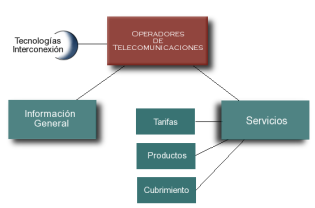
\includegraphics[width=80mm, height=52mm]{operadores.png}
 \caption{Arquitectura Básica del Subsistema Operadores de Telecomunicaciones}
 \label{operadores}
\end{figure}

Contiene información relacionada con operadores de telecomunicaciones, figura \ref{operadores}, con énfasis en las características técnicas de los servicios que ofrecen, su cobertura y tarifas. Brinda a los analistas información comparativa entre operadores lo que permite determinar las ventajas y desventajas entre diferentes opciones de interconexión, de acuerdo a los servicios médicos que se quieren implementar. Este módulo se complementa con la información de los subsistemas de tecnologías de interconexión y servicios médicos, así como de la información de dominio público que muestra el \textit{Sistema de Información Unificado para el sector de las Telecomunicaciones} mantenido por la Comisión Reguladora de Telecomunicaciones.

\subsection{Subsistema Organizaciones y Proyectos} 

Posee herramientas informáticas para la gestión de información de proyectos nacionales y de la región en el ámbito de la Telemedicina, la Telesalud y la Tele - educación en medicina. 

Incluye secciones para la gestión de los datos correspondientes a organizaciones y grupos de investigación que trabajen en el área de la Telemedicina.  Este subsistema es uno de los pilares del SITEM pues en él se despliegan aplicaciones que fomentan el trabajo en grupo y se realiza la captura de las experiencias adquiridas en los diferentes proyectos desarrollados en el área. Así mismo el módulo posee herramientas de edición que permiten la sincronización del trabajo en la realización de estudios de factibilidad y estudios técnicos.

En la actualidad se está desarrollando la opción de generar automáticamente matrices comparativas sobre criterios predefinidos, lo que brinda una fuente de información para el seguimiento de buenas prácticas en el desarrollo de proyectos en el área.

\subsection{Subsistema Servicios Médicos} 
Este subsistema cuya arquitectura se muestra en la figura \ref{servicios}, contiene una guía catalogada de los diferentes servicios y especialidades médicas disponibles. Se pone especial atención en la descripción detallada de los requerimientos técnicos y tecnológicos que requiere cada especialidad así como el perfil de los profesionales y entidades educativas de formación de especialistas. Algunos componentes de este subsistema permiten la gestión de información - con base en la normatividad colombiana e internacional, relativa a procedimientos, medicamentos, enfermedades, laboratorios, etc. Esto lo convierte en un elemento de apoyo de una plataforma de servicios como puede ser la de consulta remota, el telediagnóstico o la tele - educación médica.

\begin{figure}
 \centering
 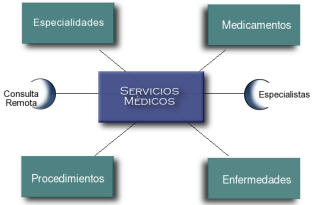
\includegraphics[width=80mm, height=60mm]{servicios.png}
 \caption{Subsistema Servicios Médicos}
 \label{servicios}
\end{figure}

\subsection{Subsistemas Entornos de Aprendizaje} 
Siguiendo la filosofía de integración del SITEM a proyectos de software libre, el subsistema de entornos de aprendizaje incorpora y adapta los elementos de la plataforma \textbf{Moodle} y provee un ambiente en línea para la estructuración, mantenimiento y distribución de conocimiento a través de cursos y seminarios. 

El subsistema permite libre acceso de usuarios a un conjunto de cursos y seminarios que apoyan el desarrollo de competencias en el área de la teleinformática, la telesalud, la telemedicina, las tecnologías de la información y las comunicaciones. Con un enfoque constructivista se procura la retroalimentación de los contenidos por parte de la comunidad. 

Como patrón de desarrollo el SITEM integra a su arquitectura, figura \ref{aplicaciones_sitem}, soluciones exitosas y robustas en el mundo del software libre, de esta forma reutiliza gran cantidad de aplicaciones, las adapta para proveer un ambiente integrado y aumenta sus prestaciones para implementar nuevos casos de uso. Entre las aplicaciones, mostradas en la figura \ref{aplicaciones_sitem}, que contribuyen enormemente en el SITEM se pueden citar:

\begin{description}
 \item[Moodle] Es un ambiente integrado de aplicaciones para la creación, organización, mantenimiento y seguimiento de cursos en línea. El fin primordial de sus herramientas es dar soporte a un marco de educación social constructivista.

\item[PHPBB] Conjunto de módulos escritos en PHP y Python para la gestión de foros en línea; aunque su línea funcional base hace parte de Moodle, en el SITEM los foros de carácter general - aquellos que no pertenecen a un entorno de aprendizaje específico, se implementan usando PHPBB. El manejo de sesiones, la gestión de usuario y la autenticación se han recodificado para que sean compatibles con los subsistemas principales del SITEM.

\item[MediaWiki] Herramienta para la construcción de sitios web tipo Wiki. Un Wiki es un neologismo basado en un término hawaiano y hace referencia a un sitio en el cual el contenido se construye de forma colaborativa usando para ello un lenguaje de etiquetado intermedio que permite la aplicación de cierta plantillas a porciones de texto para poder darles un formato específico. Aunque la información de una página Wiki no esta estructurada, el sistema lleva un historial de cambios por lo que será posible reconstruir el estado de dicha página en cualquier momento de su vida. Este aplicativo esta siendo usado en el SITEM para la construcción de su enciclopedia, los manuales de usuario y en ciertos módulos que requieren la construcción colaborativa de contenidos.

\item[MapServer] Es una aplicación desarrollada en Python que proporciona al SITEM los servicios básicos necesarios para la georeferenciación de la información en el subsistema de consultoría. La plataforma de MapServer define un conjunto de bibliotecas que permiten el manejo de información geográfica. Es software libre y soporta entre otros los formatos: ESRI shapefiles, PostGIS, ESRI ArcSDE, GML; utilizando la librería OGR (http://www.gdal.org/ogr/, 2007).

\item[Google] Su servicio web de motor de búsqueda se usa en el SITEM. Esta es una solución parcial que a corto plazo será desplazada por herramientas de software libre tales como DataparkSearch (http://www.dataparksearch.org/, 2007), ASPSeek (http://www.aspseek.com) y algunas bibliotecas en desarrollo por los integrantes del GITEM.

\item[Sistema de Información Unificado del Sector de Telecomunicaciones] Conocido como SIUST, es un aplicativo Web desarrollado por la Comisión Reguladora de Telecomunicaciones que contiene información del sector de las telecomunicaciones en Colombia: “...información técnica de infraestructura, normatividad del sector, estadísticas comerciales e índices financieros de los prestadores de servicios y los indicadores de gestión del sector entre otros.” \footnote{Tomado del sitio web del SIUST. http://www.siust.gov.co/siust/}

La información, que es de acceso público, permite que el SITEM se nutra de ella para complementar y validar sus propias bases de datos en algunos subsistemas.

\item[Wikipedia] Quizás la fuente de información colaborativa más grande en Internet, debido a que sus contenidos son de uso libre, el SITEM se nutre de ellos y a su vez los complementa. A partir de información disponible se han editado más de 50 artículos en Wikipedia que tienen relación temática con el SITEM.

 \end{description}

\begin{figure}
 \centering
 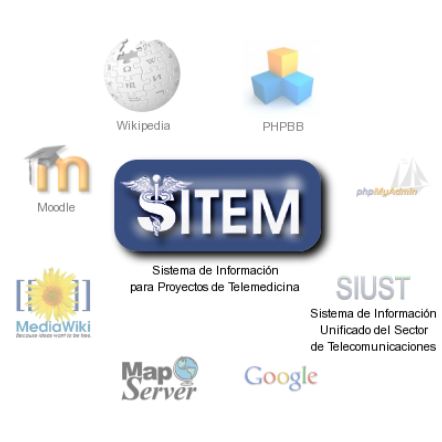
\includegraphics[width=156mm, height=156mm]{sitem_aplicaciones.png}
 \caption{Aplicaciones de Software Libre o Uso libre que complementan al SITEM}
 \label{aplicaciones_sitem}
\end{figure}

Es un objetivo claro del proyecto la integración con otros productos de software libre promoviendo el uso de tales herramientas, el desplazamiento del mercado hacia soluciones basadas en productos de código abierto como estrategia válida para el despliegue de aplicaciones en Telemedicina en entidades que tengan bajos recursos para el montaje y mantenimiento de redes de atención soportas en TIC.

\section {Aspectos Relativos a la Fase de Transición}

El actual despliegue de la solución en una plataforma tecnológica adecuada tal como se muestra en el anexo \ref{modelo_despliegue}, garantiza un óptimo servicio a los potenciales usuarios \footnote{La versión actual esta disponible en Internet en la dirección http://gitem.udistrital.edu.co/sitem/} y marca el paso de la versión 3.0 del producto a la fase de transición. Las herramientas básicas se encuentran disponibles para que el grupo de investigación convoque a las entidades de salud, profesionales en el área de la tecnología, especialistas en medicina y fabricantes - distribuidores - de dispositivos médicos que participaron en la primera fase del Estudio Red de Telemedicina Bogotá \cite{aparicio2000} para que de forma conjunta enriquezcan la base de información en el subproceso de prueba piloto.

Basado en el módulo de generación de herramientas para la recolección de información, anexo \ref{manual_usuario}, el grupo aplicará diferentes instrumentos entre los que se incluyen:

\begin{itemize}
\item Entrevistas: Con el objeto de acordar las directrices a seguir tanto con los operadores de telecomunicaciones, como los prestadores del servicio de salud que participaron de la fase I de recolección de información con el propósito de socializar los resultados del proyecto e invitarlos para que editen y actualicen sus datos obteniendo beneficios incrementalmente. Dichos servicios van desde la disponibilidad de un mapa de sedes, servicios y profesionales hasta la consolidación de información para la gestión de sus redes tecnológicas primarias.

\item Encuestas: Para identificar nuevos requerimientos de servicios que puedan ser desplegados en la plataforma propuesta. Además, estos instrumentos permitirán medir el impacto en la cobertura de los servicios y de participación de las instituciones objeto de la investigación de campo.
\end{itemize}

Las unidades de recolección de información mostradas en el anexo \ref{formulario_preliminar}, se han adaptado de aquellas propuestas por el proyecto europeo HERMES. \footnote{Proyecto de investigación a tres años, financiado por la Comunidad Económica Europea y que cumplió sus objetivos hacia principios del milenio dejando como resultado un conjunto de preguntas básicas que apoyan los procesos de implementación de soluciones médicas apoyadas en las TIC.} El modelo investigación evaluativa que continua en la fase IV del proyecto pretende medir la evolución del nivel de servicios de salud prestados con el apoyo de TIC comparando sucesivamente el modo de operación encontrado entre el año 2000 y 2005 con aquel encontrado entre el año 2008 y 2011 luego que algunas entidades interactúen con el SITEM.

\subsection {Fuentes de Información Primaria}

Para la carga de información inicial en el SITEM se utilizan los resultados del estudio de campo realizado en varias instituciones de carácter público y privado. Dicho resultados se encuentran consignados en sendas tesis en formato digital e impresos disponibles en la biblioteca de la Universidad Distrital y archivo del grupo de investigación:

\begin{itemize}
 \item Hospital Rafael Uribe Uribe.\cite{guarin2003}
 \item Hospital San Pedro Claver.\cite{ardila2001},\cite{rozo2002}
 \item Hospital Simón Bolívar. \cite{acero2002}
 \item Hospital El Tunal. \cite{ruiz2002}\cite{duque2002}
 \item Hospital La Victoria.\cite{barrero2000}
 \item Hospital San José.\cite{gonzalez2002}
\end{itemize}